\section{Summary}

The work within previous chapters have demonstrated the power of lens modeling as a tool for uncovering the mysteries of the high redshift universe. The Frontier Fields lens models have provided the community with easily-accessible lensing information of all the clusters for a variety of researchers regardless of their own expertise in lensing. Many of the Frontier Fields lens modeling papers in the literature, including that of the work in Chapter~\ref{chap:hff_clusters}, have been cited over 100 times since the models were released in 2014 \citep{Johnson:2014tg,Richard:2014gf}. This work includes greatly improving constraints on the faint end of luminosity functions at $z\sim6$ \citep {Bouwens:2017df} as well as extending the luminosity function out to $z\sim10$ \citep{Ishigaki:2017le,Ishigaki:2015cs,McLeod:2016xw}. Additional studies include characterizing the size distribution of these high redshift galaxies \citep{Kawamata:2017bc, Bouwens:2017to,Kawamata:2015ax}, as well as work on the clusters themselves, including intracluster light \citep{Montes:2018hs,Montes:2014jx,Morishita:2017zf} and dark matter substructure \citep{Natarajan:2017qp,Jauzac:2016dn,Mohammed:2016bk,Grillo:2016jk}. Another exciting discovery has been Supernova Refsdal, which was multiply-imaged into an Einstein cross in a galaxy at $z\sim1.5$ by both the cluster \MACSeleven\ and one of its galaxies \citep{Kelly:2016az,Rodney:2016sf,Kelly:2015pj}. With the lens models, astronomers were able to accurately predict a supernova \citep{Treu:2016lr,Jauzac:2016ux,Sharon:2015xe,Oguri:2015hb} -- Refsdal reappeared in another image of the galaxy roughly a year later \citep{Kelly:2016hw}.

We have seen, in Chapter~\ref{chap:ares_systematics} that due to the wealth of constraints and spectroscopic information, the Frontier Fields lens models are less vulnerable to systematic errors in derived magnifications \citep{Johnson:2016rt}. When marginalizing over the results produced by different modeling techniques, scientists can account for the systematic errors in the modeling methods themselves \citep{Meneghetti:2016xe}. \citet{Acebron:2017wl} also find that cosmological parameters can be retrieved from lens models of clusters similar to the Frontier Fields.

We have also seen how lensing clusters can magnify background galaxies to allow for unique, high resolution studies of galaxies at $1<z<3$. We saw in the modeling of \cluster\ that it is possible to break the kiloparsec, even the centaparsec resolution barrier in a galaxy at $z\sim2.5$. This result has major implications for understanding the morphologies of galaxies at cosmic noon. \citet{Rigby:2017qy} show that if \giantarc\ had been observed with \hst\ in a survey such as CANDELS or even in the HUDF, it would not be classified as a ``clumpy" galaxy as we see it lensed. We see with lensing that roughly a quarter of the star formation in \giantarc\ occurs in what we classify as clumps, where as in the hypothetical case this galaxy were observed in a deep field, we would see all the star formation occurring in an exponential disk (see Figure~\ref{conc:fig:candelized}).

And in Chapter~\ref{chap:sim}, we have seen how vulnerable the derived mass and magnifications of clusters with few constraints are to systematic errors. These errors may be sensitive to the exact image configurations or even the redshift distributions of the sources.

\begin{figure}
\centering
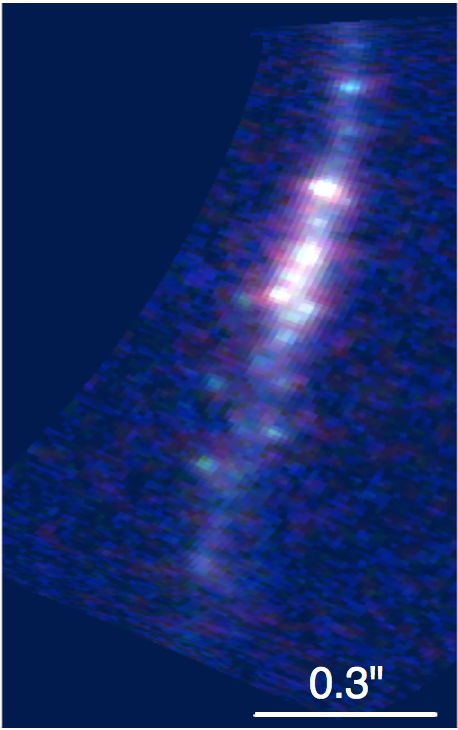
\includegraphics[height=0.4\textheight]{Conclusion/candelized_highres.png}
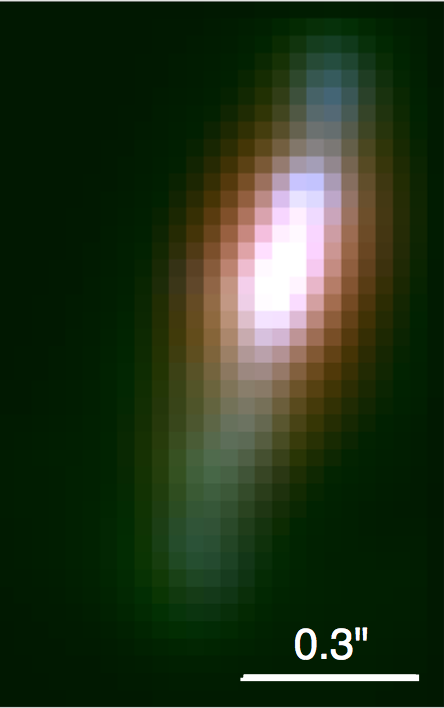
\includegraphics[height=0.4\textheight]{Conclusion/candelized_lowres.png}
\caption[Comparison of lensed \giantarc\ source reconstruction to its unlensed deep field realization]{From \citet{Rigby:2017qy}: (Left) The source plane reconstruction of \giantarc, pixel scale of 3 mas. Roughly 24\% of the star formation of this galaxy is in clumps. (Right) \giantarc\ source reconstruction convolved with the \hst\ PSF and rebinned to a pixel scale of 30 mas. This is what this galaxy would look like had it been detected in a deep field. All the star formation would be observed to occur in an exponential disk, with no evidence of clump morphology.}
\label{conc:fig:candelized}
\end{figure}

\section{Future of cluster lensing}

The Frontier Fields are only six unique sight lines to some of the best lensing clusters in the sky with full wavelength coverage in imaging and spectra. Despite their usefulness in characterizing the formation of galaxies into the era of cosmic re-ionization and understanding systematics of lens modeling techniques, the future of lensing will not depend on a handful clusters, but rather thousands.

\subsection{Clusters in future surveys}

As mentioned before, several hundreds of strong lensing clusters have already been discovered in ground-based optical surveys like SDSS and DES as well as in optical follow-up by surveys such as ROSAT, Planck, ACT, and SPT. The vast majority of these clusters have been discovered based on their high magnifications of background objects into discernible giant arcs. As on-going studies of these lensing systems are taking place, the astronomical community is greatly anticipating the first light from several new ground- and space-based optical observatories. The {\it Large Synoptic Survey Telescope} \citep[{\it LSST}; ][]{IVezic:2008tv} is expected to have first light in 2020 and will likely find hundreds of strong lensing clusters as it images entire southern sky every few nights. The National Aeronautics and Space Administration (NASA) plans to launch the {\it Wide Field Infrared Survey Telescope} \citep[{\it WFIRST}; ][]{Spergel:2013zk}, a 2.4-m infrared space telescope that will survey much of the sky and plans to find $>$40,000 galaxy clusters, but with roughly the same resolution as \hst. {\it WFIRST} is currently on-track to be launched in the 2020s. A complementary mission to {\it WFIRST} in the optical will be the European Space Agency's (ESA) {\it Euclid} telescope \citep{Laureijs:2011qt}, a 1.2-m telescope with a launch date planned for 2021. {\it Euclid} plans to identify $\sim10^5$ strong lensing systems.

\subsection{Modeling the lenses found in surveys}

As the previous chapters have demonstrated, robust lens models require many multiple images with spectroscopic redshifts. However, the lensing systems found in large field surveys typically have one or two highly magnified sources which can be identified from ground-based imaging. Perhaps with space-based imaging, more image systems can be detected as the higher resolution makes it easier to match multiple images based on color and morphology. However, the galaxy clusters found in these surveys are likely to be average in mass and therefore will only have cross-sections large enough to multiply image a handful to perhaps a half dozen background sources. Additionally, since these surveys are imaging only, obtaining redshifts for the background sources is mostly limited to photometric redshift information (which may be inaccurate due few photometric bands). Obtaining any spectroscopic redshifts will be expensive in terms of hours of integration spent on large ground-based telescopes. Some of images might even be too faint or not have emission lines in the optical which can be detected or may lie in the redshift desert for the instrument.

Due to the dearth of lensing information, creating robust lens models for these clusters will be extremely difficult. While much work has been done to quantify systematics for the Frontier Fields clusters, little to no work has been done to quantify systematics of any sort on clusters with fewer than five multiple image systems. It is expected for these systems to be highly prone to systematic errors as there is poor sampling of the potential.

Additionally, modeling thousands of clusters is currently a difficult task to pursue. At the moment, each cluster model is modeled with individual care. While it may be possible to automate the selection of cluster member galaxies using photometric cuts, the data needs to be thorough inspected for multiple images by eye. And as obtaining spectroscopy is expensive in terms of telescope time, careful discretion needs to be exercised in terms of prioritizing which images are targeted for spectroscopic follow-up.

\section{Final Remarks}

While many arduous tasks lie ahead for the lens modeling community in terms of fully understanding the systematics of the models created, the future is bright. The thousands of strong lensing systems will provide astronomers with many suitable targets for high resolution telescopes like \hst\ and {\it JWST}, or even the {\it Atacama Large Submillimeter/Meter Array} ({\it ALMA}). These galaxies at $z\sim2$ are forming during the time in the Universe's history when star formation was at its peak. Typical galaxies from this era will evolve into galaxies not unlike our own, so strong lensing holds to the key to pursuing a kind of ``stellar archeology" on our own galaxy.

Additionally, massive galaxy clusters will be our best sight lines to finding the first galaxies formed in the Universe. Obtaining SEDs of these galaxies will help us to understanding the properties of the first generation of stars (Population I), for which we still are uncertain of their formation given their low metallicity environments. Furthermore, finding many of these distant galaxies will allow us to measure the overall UV luminosity function, which will tell us how the Universe was able to re-ionize itself after the Big Bang.

This dissertation presents some of the pioneering work that will shape the lensing science to come. Making lens models public has allowed for many researchers from different backgrounds to pursue interesting science without having to know the {\it in's and out's} of lens modeling and is a practice that should be continued to allow for collaborative work in the future. My work on \giantarc\ shows the usefulness of cluster lensing for high-resolution star formation studies and how our forward modeling technique can greatly benefit these studies by allowing for a deconvolution of the source reconstruction from the lensing PSF. Finally, I have begun to quantify the systematics of strong lensing and demonstrated the need to look to simulations to fully understand the accuracy in lens modeling during the era of precision lensing.


